% LLNCStmpl.tex
% Template file to use for LLNCS papers prepared in LaTeX
%websites for more information: http://www.springer.com
%http://www.springer.com/lncs

\documentclass{llncs}
%Use this line instead if you want to use running heads (i.e. headers on each page):
%\documentclass[runningheads]{llncs}
\usepackage{algorithm,algorithmic,amsmath,comment,listings,color,graphicx, float}

\definecolor{dkgreen}{rgb}{0,0.6,0}
\definecolor{gray}{rgb}{0.5,0.5,0.5}
\definecolor{mauve}{rgb}{0.58,0,0.82}

\lstset{frame=tb,
  language=C,
  aboveskip=3mm,
  belowskip=3mm,
  showstringspaces=false,
  columns=flexible,
  basicstyle={\small\ttfamily},
  numbers=none,
  numberstyle=\tiny\color{gray},
  keywordstyle=\color{blue},
  commentstyle=\color{dkgreen},
  stringstyle=\color{mauve},
  breaklines=true,
  breakatwhitespace=true,
  tabsize=3
}

\begin{document}
\title{Rate-based Synchronous Diffusion}

%If you're using runningheads you can add an abreviated title for the running head on odd pages using the following
%\titlerunning{abreviated title goes here}
%and an alternative title for the table of contents:
%\toctitle{table of contents title}

\subtitle{Internet of Things}

%For a single author
%\author{Author Name}

%For multiple authors:
\author{Balz Aschwanden, David Boesiger, Jovana Micic,  Raoul Norman Grossenbacher} 


%If using runnningheads you can abbreviate the author name on even pages:
%\authorrunning{abbreviated author name}
%and you can change the author name in the table of contents
%\tocauthor{enhanced author name}

%For a single institute
%\institute{University of Bern}

% If authors are from different institutes 
\institute{University of Bern \newline \{balz.aschwanden, david.boesiger, jovana.micic, raoul.grossenbacher\}@students.unibe.ch}


%to remove your email just remove '\email{email address}'
% you can also remove the thanks footnote by removing '\thanks{Thank you to...}'


\maketitle

%\begin{abstract}
%abstract text goes here - Lorem ipsum dolor sit amet, consectetur adipiscing elit, sed do eiusmod tempor incididunt ut labore et dolore magna aliqua.
%\end{abstract}

\begin{comment}
Protocol introduction: Maximum 1 page about the theoretical basics of the experiment.
\end{comment}
\section{Protocol Introduction}
Very often time synchronization of all sensors is required in Wireless Sensor Network (WSN). Since each node has its own clock, it is  needed to synchronize clocks in order to support synchronized sleep and duty cycles among nodes.

 \textbf{Rate-Based Diffusion Protocol (RDP)} aims to synchronize the nodes in the network to the average value of the clocks in the network.
Rate-Based Diffusion Protocol has two main phases:
\begin{enumerate}
\item  Neighbourhood Discovery Phase

In this phase, each node has to periodically broadcast a packet with its ID and sequence number to get to know neighbours. All recognized neighbours are saved in neighbour table. Additionally, with each neighbour we have to save the time offset between the node's time and the neighbours times. Broadcast is determined by time the node waits after starting broadcasting. This parameter value will be discussed later in further sections. 

\item  Convergence Phase

In convergence phase, each node periodically go through neighbours table and update own time using following formula:
\[t_i= t_i -  r * (t_i-t_j)\]
Basic idea is to adapt time of the node to the neighbours node time using some r-value.
R-value needs to be $0<r<1$. Results of choosing different r-values will be discused in further sections. 
In this phase, unicast messages are used to determine the offset between the clocks.  
\end{enumerate}
\pagebreak 
Algorithm 1 is showing the pseudo code for Rate-based Diffusion Protocol. 
\begin{algorithm}
 \caption{Diffusion algorithm to synchronize the whole network}\label{euclid}
  \begin{algorithmic}[1]
    \STATE Do the following with some given frequency
    \FOR{each sensor $n_i$ in the network}
     \STATE Exchange clock times with $n_i$'s neighbours
      \FOR{each neighbour $n_j$}
        \STATE Let the time difference between $n_i$ and $n_j$ be $t_i$ - $t_j$
        \STATE Change $n_i$'s time to $t_i$-$r_ij$($t_i$-$t_j$)
      \ENDFOR
    \ENDFOR
\end{algorithmic}
\end{algorithm}

\begin{comment}
Methods: especially, describe the methods used to realize the protocol
(functions in the code and their functionality).
\end{comment}
\section{Methods}
In the following part we will show implemented code for receiving and sending unicast messages. The algorithm is very similar to RTT synchronization. A unicast message in our code contains the following variables:
\begin{itemize}
	\item a boolean to know if the message has passed one round
	\item the ids of sender and receiver
	\item the clock time values of both nodes
\end{itemize}
First the clock time from the sender is inserted and the message is sent to a neighbour. That neighbour then inserts its time change the boolean and sends the packet back. The code is equivalent to the above expect the following lines. The send\_uc method is used for both: 

\begin{lstlisting}
static void send_uc(uint8_t receiverId, clock_time_t receiverTime, uint8_t isRequestForTime) {
	rimeaddr_t addr;
	static struct unicastMessage ucReply;
	ucReply.senderId = node_id;
	ucReply.senderTime = clock_time();
	ucReply.receiverTime = receiverTime;
	ucReply.isRequestForTime = isRequestForTime;

	addr.u8[0] = receiverId;
	addr.u8[1] = 0;
	packetbuf_copyfrom(&ucReply, sizeof(ucReply));
	unicast_send(&ucConn, &addr);
}
\end{lstlisting}

 Then the offset the that neighbour is calculated and saved into the neighbour table. To calculate this offset we simply add half of the RTT to the neighbour time we receive back and compare it to our own time. 

\begin{lstlisting}
static clock_time_t calc_offset(clock_time_t senderTime, clock_time_t receiverTimeOld)
{
    clock_time_t curr = clock_time();
    clock_time_t rtt = curr - receiverTimeOld;
    clock_time_t neighborTime = senderTime + rtt/2;
    clock_time_t offset = curr - neighborTime;
    return offset;
}
\end{lstlisting}

After a certain waiting for a certain time to make sure to receive all unicasts back, the sum off all offsets is calculated, multiplicated with the r-value and substracted from the clock time. This way the clock time needs to be adjusted only once per round.

\begin{lstlisting}
static void converge(int numIter)
{
	clock_time_t offset = 0;
	static int i;
	for (i = 0; i < neighborArrayOccupied; i++) {
		offset += neighborTable[i].offset;
		neighborTable[i].offset = 0;
	}

	clock_time_t newtime = clock_time() - (int) offset * rMultiplier / rDevider;
	clock_set(newtime);
}

\end{lstlisting}

\begin{comment}
Experimental setup/Measurement procedure: The experimental setup, the
differences of the experimental series, the different parameters used, including local
sensor setup and TARWIS testbed.
\end{comment}
\section{Experimental setup}
There were two phases of experiment. In the first phase we tested our program using Telos nodes and in the second phase we uploaded our code to TARWIS platform. We tried different values for\textit{r-value}, the \textit{unicast interval} as well as the \textit{broadcast interval}. In addition, we run the code with different MAC protocols. In the first version of the program we used default NullMAC protocol and in the second we used X-MAC protocol. 

By protocol algorithm, \textit{r-value} needs to be value from range of zero to one. We chose to test our code for five different r-values: 0.25, 0.5, and 0.75. 

For \textit{unicast interval} value we chose values from 5 to 10 seconds.

\begin{comment}
Results and Analysis: Analyse the results which are obtained by local sensors and
on TARWIS testbed. Analyse your data with respect to the aim of the experiment. Your
task during the experiment is not just to measure and document your measurements, but
to derive and present conclusions from your measurements.
\end{comment}

\section{Results and Analysis}

The final results showed that and \textit{r-value} of 0.5 is optimal though there were 3 nodes not responding to the algorithm when testing with 40 nodes.
\begin{figure}[H]
  \centering
  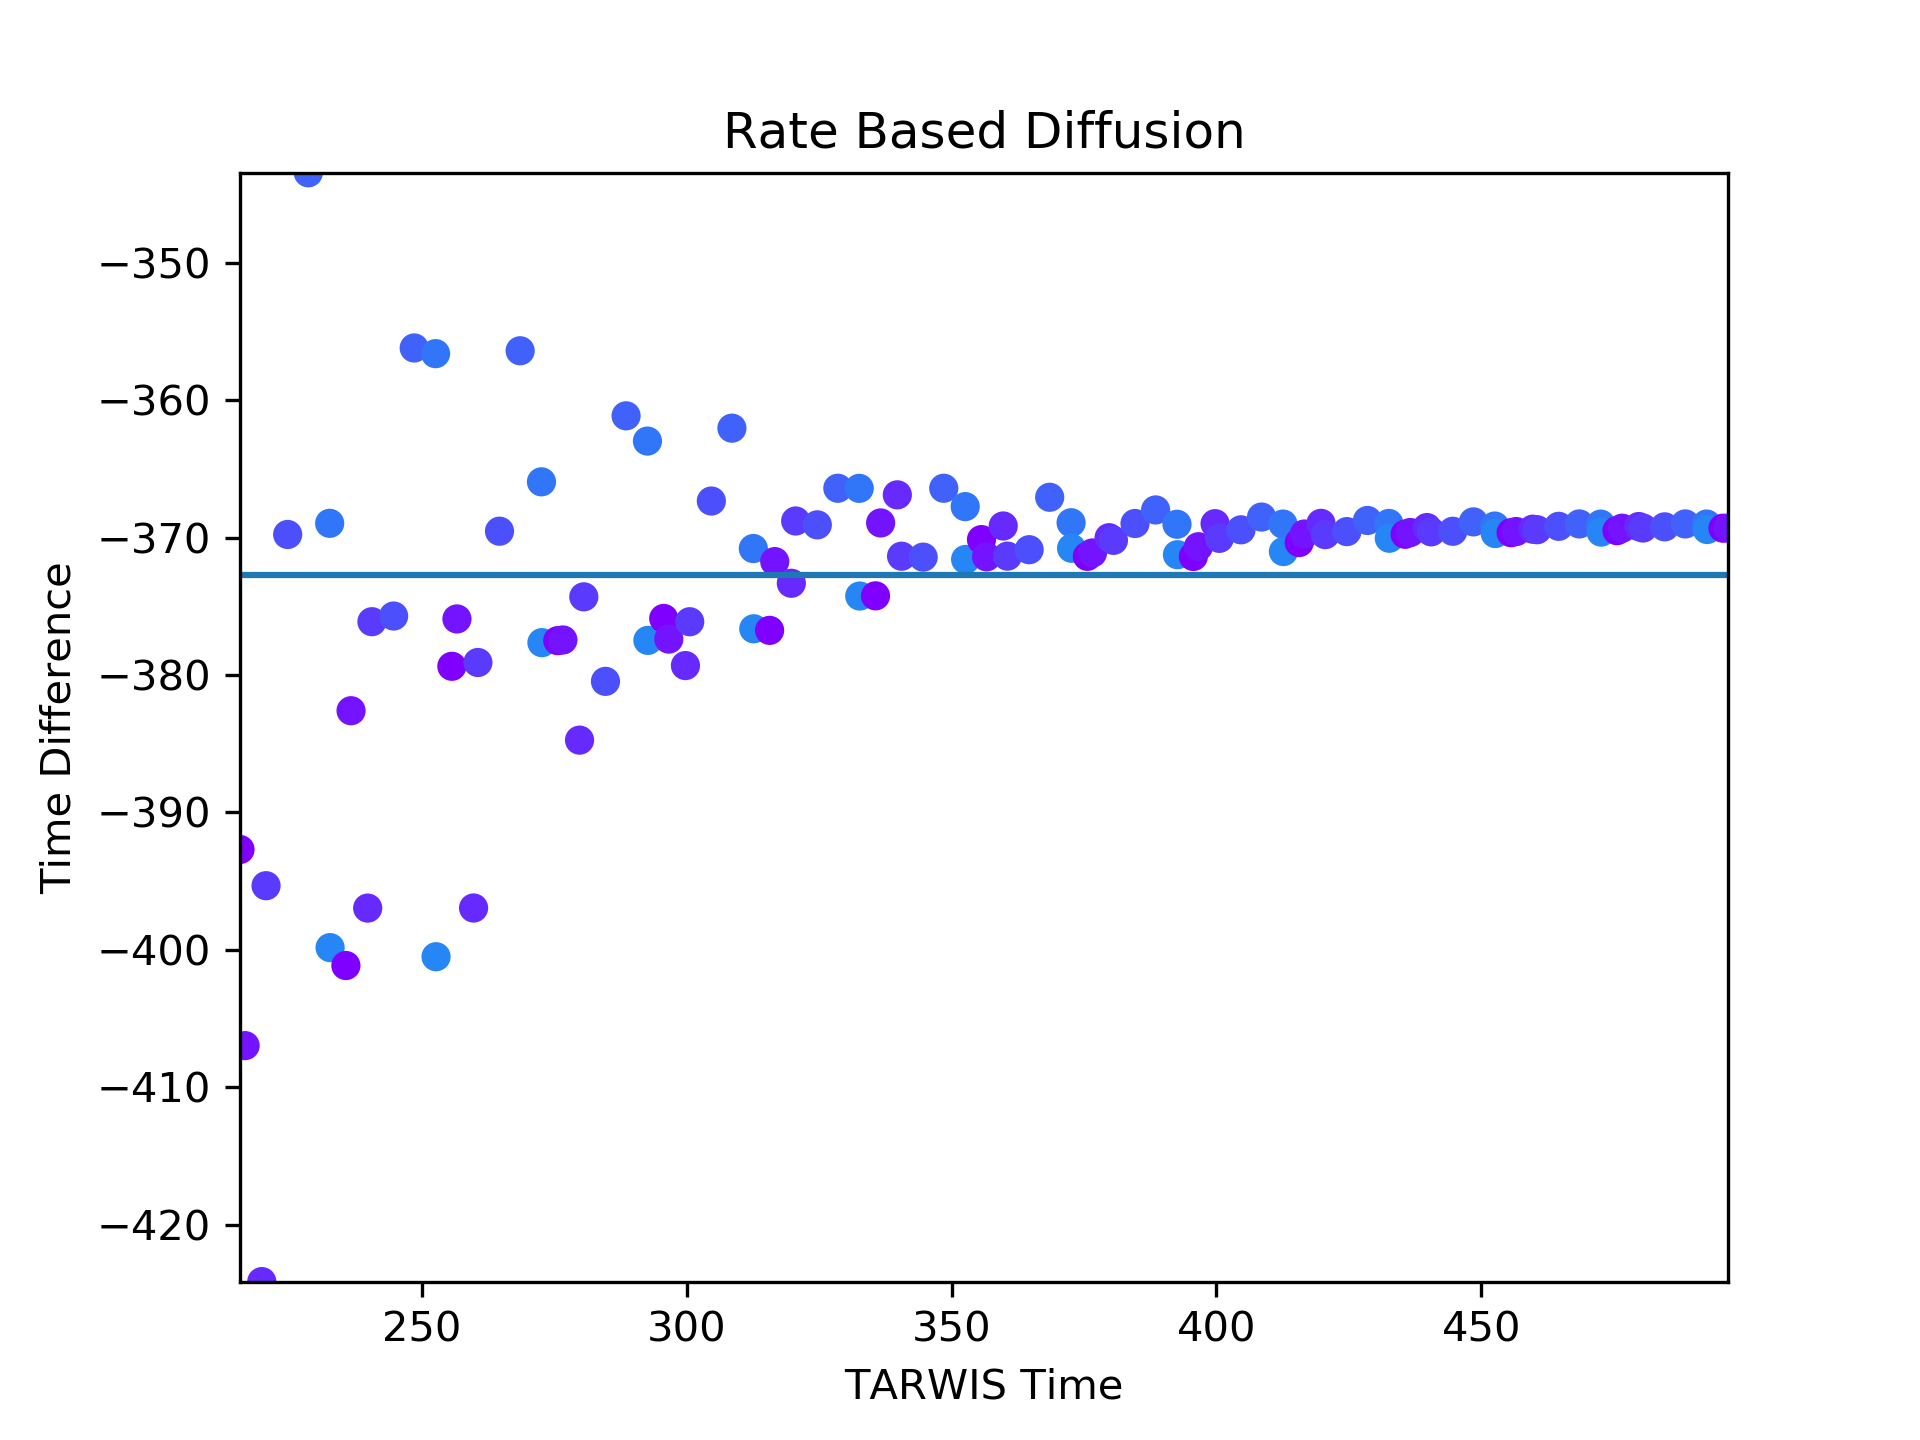
\includegraphics[width=\linewidth]{05_10.png}
  \caption{Test with $r=0.5$ ,both intervals $10$s, with $10$ nodes}
  \label{fig:Test with 10 Nodes}
  
  \centering
  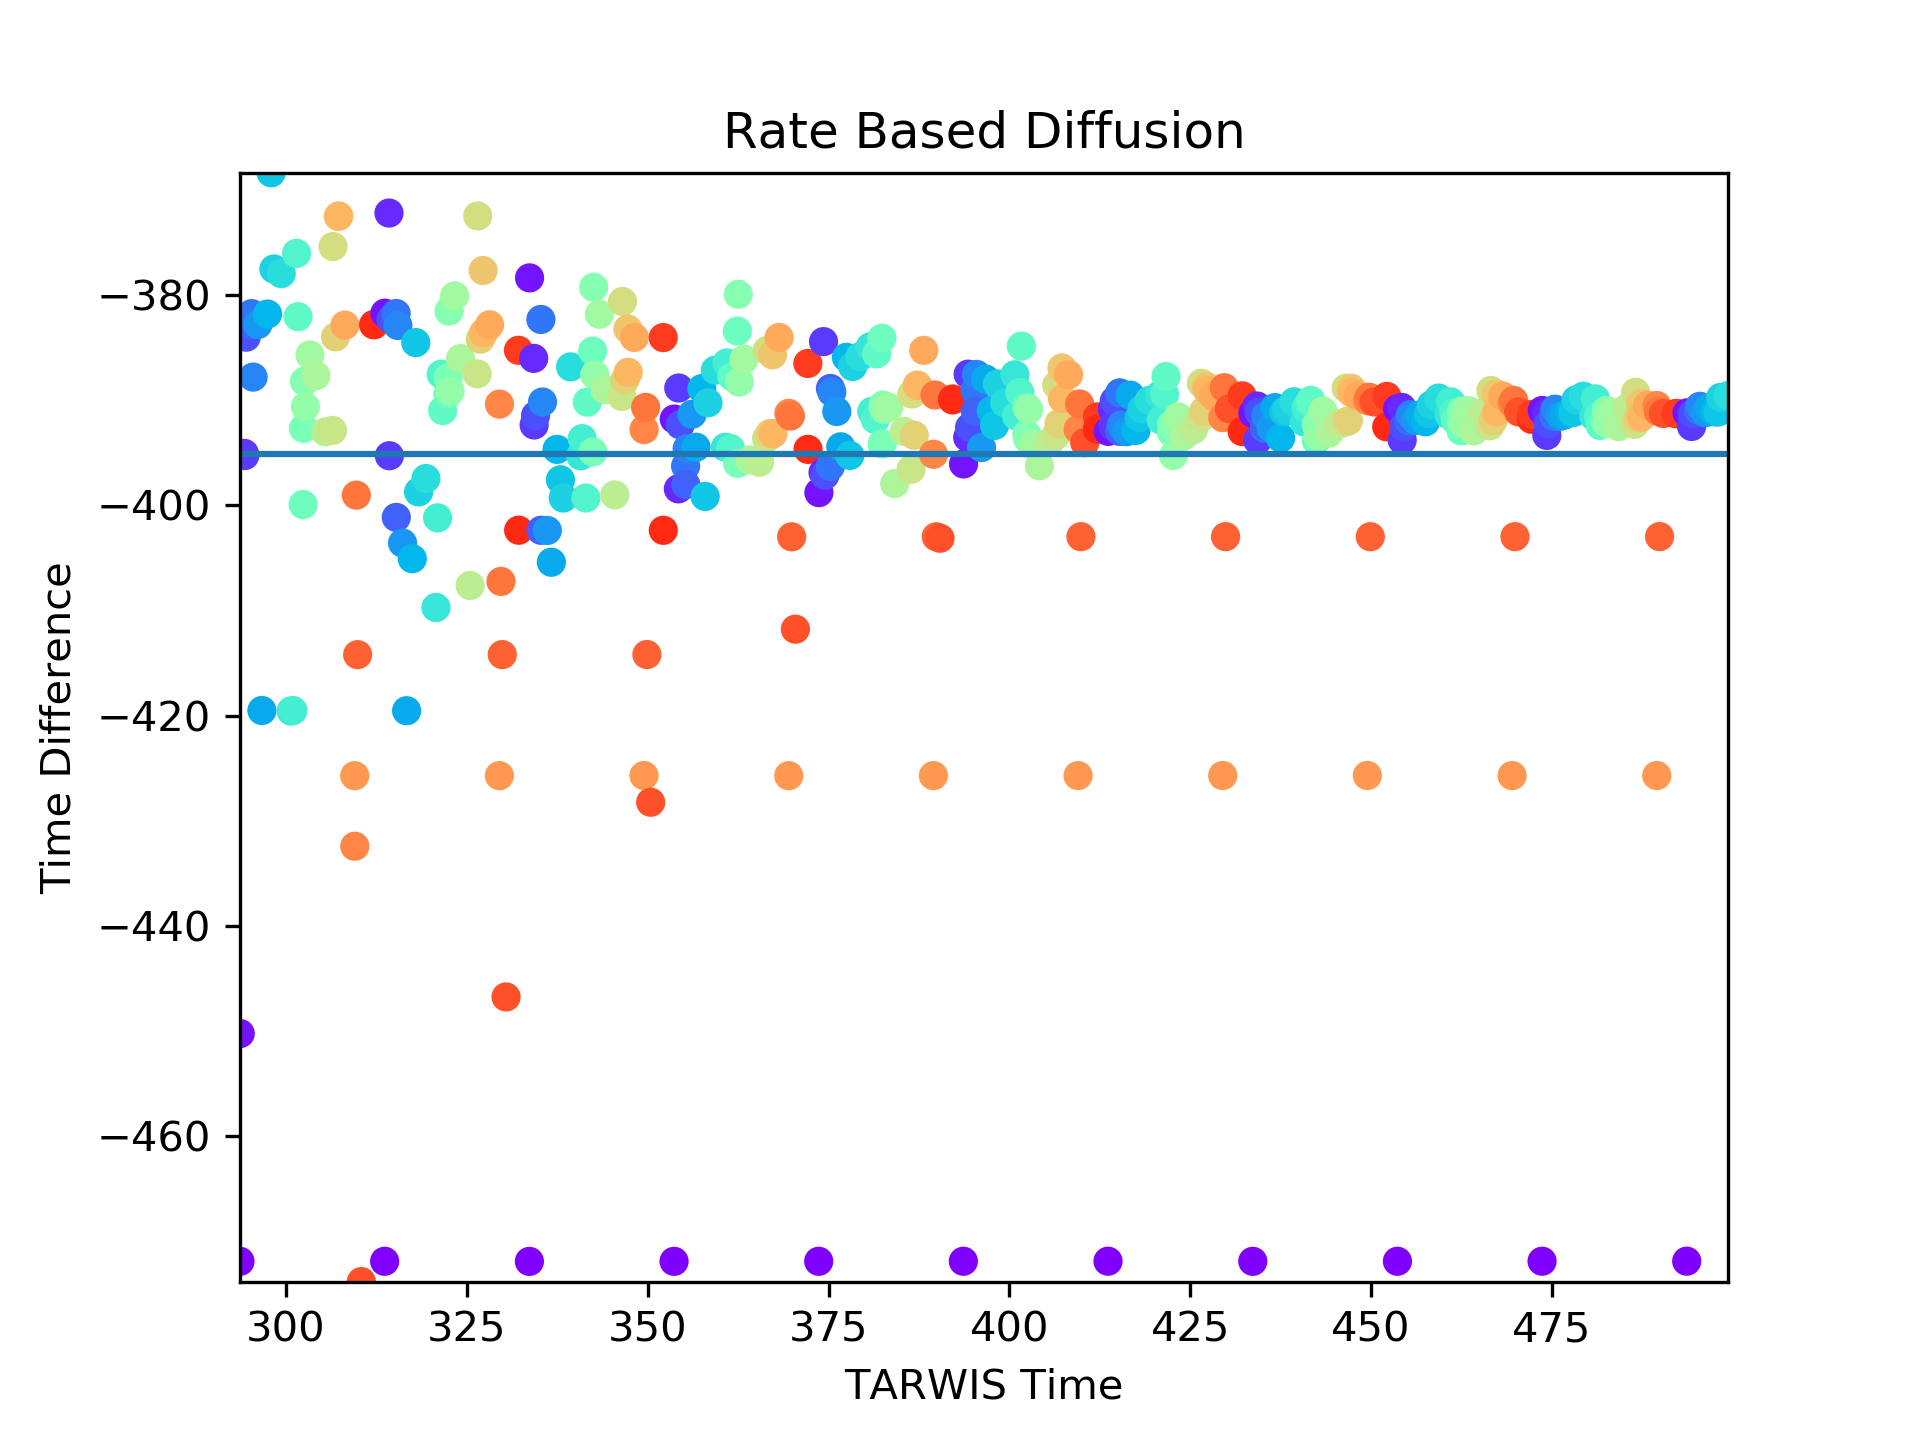
\includegraphics[width=\linewidth]{05_10_40.png}
  \caption{Test with $r=0.5$ ,both intervals $10$s, with $40$ nodes}
  \label{fig:Test with 40 Nodes}
\end{figure}

In these charts the time difference is the difference between the node time and the TARWIS time. The TARWIS time thus represents some global reference. You can also see a line which is the mean over all measurements.

At first a time interval of 10 Seconds was chosen for both intervals. Later on there were tests with lower time intervals though the result weren't satisfying,
so the time intervals were kept during all tests. 
For r-values smaller than 0.5 the conversion still was happening, but at a slower rate.
If the r-value was over 0.5 there was no visible conversion in the charts.
When testing with XMAC, no node was responding to one another. 
This was probably because the nodes weren't able to build their neighbour table, or they did not pick up the unicasts from their neighbours, thus they were not able to send them back and the offsets would stay to 0 for each neighbour, so the clock won't change.


\begin{figure}[H]
  \centering
  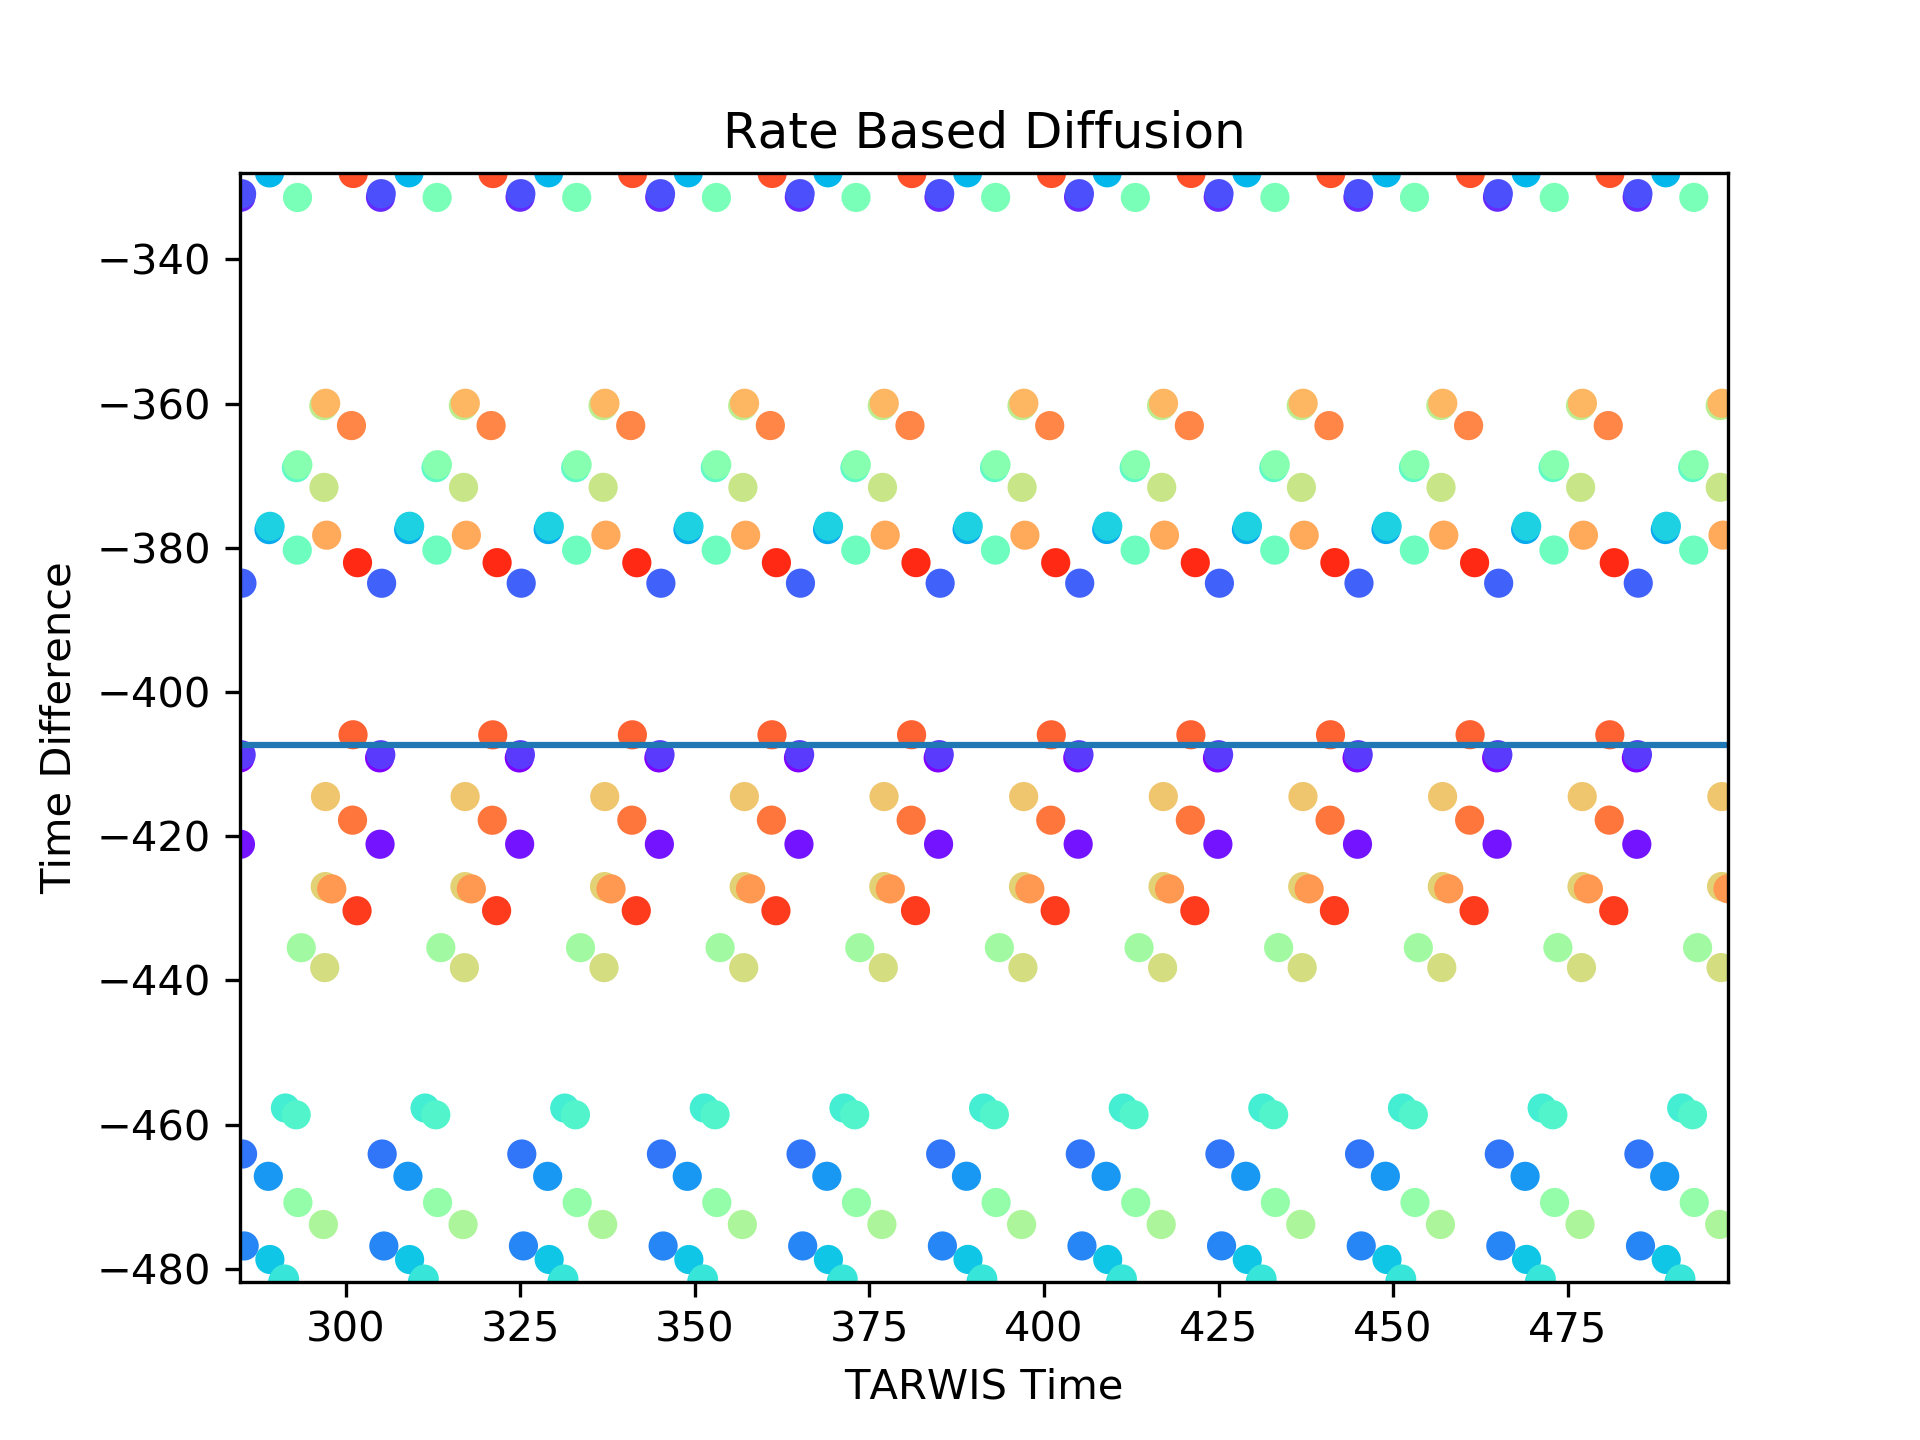
\includegraphics[width=\linewidth]{xmac.png}
  \caption{Test with Xmac}
  \label{fig:Test xmac}
\end{figure}

It makes intuitively sense that an r-value of 0.5 would show the best results which was confirmed by our test.


\begin{comment}
Conclusions: Summarize and discuss your results with respect to the literature or
your own scientific expectations. You should in particular discuss possible error sources
and give a short judgement on the quality of the experimental setup (because you also
learn to design the measurement setups). If needed, suggest how to improve the setups.
\end{comment}

\section{Conclusions}

There are a lot of challenges when implementing this algorithm. First of all it is difficult to find good times for the both intervals since conditions like environment can change every time, theses intervals ideally need to be different every time. Second there were also technical challenges. The clock time for example only has a certain range and switches from its highest value to its lowest value when overflowing and vice versa. When working with such nodes it is essential to know those things in order to succeed. In light of that the results were more or less as expected.

\subsection{Improvements}
Even though the synchronization worked well, there are still a lot of improvements that could be made. 
For example the clock time is not taken into consideration in the code.
Further the calculation for the offset is done with integers, so rounding errors could occur. 
If there are a lot of unicast messages sent at one point, packets may be lost resulting in a slower performance of the algorithm.




%The bibliography, done here without a bib file
%This is the old BibTeX style for use with llncs.cls
\bibliographystyle{splncs}

%Alternative bibliography styles:
%the following does the same as above except with alphabetic sorting
%\bibliographystyle{splncs_srt}
%the following is the current LNCS BibTex with alphabetic sorting
%\bibliographystyle{splncs03}
%If you want to use a different BibTex style include [oribibl] in the document class line

%\begin{thebibliography}{1}
%add each reference in here like this:
%\bibitem[RE1]{reference1}
%Author:
%Article/Book:
%Other info: (date) page numbers.
%\end{thebibliography}

\end{document}

